%
% FH Technikum Wien
% !TEX encoding = UTF-8 Unicode
%
% Erstellung von Master- und Bachelorarbeiten an der FH Technikum Wien mit Hilfe von LaTeX und der Klasse TWBOOK
%
% Um ein eigenes Dokument zu erstellen, müssen Sie folgendes ergänzen:
% 1) Mit \documentclass[..] einstellen: Master- oder Bachelorarbeit, Studiengang und Sprache
% 2) Mit \newcommand{\FHTWCitationType}.. Zitierstandard festlegen (wird in der Regel vom Studiengang vorgegeben - bitte erfragen)
% 3) Deckblatt, Kurzfassung, etc. ausfüllen
% 4) und die Arbeit schreiben (die verwendeten Literaturquellen in Literatur.bib eintragen)
%
% Getestet mit TeXstudio mit Zeichenkodierung ISO-8859-1 (=ansinew/latin1) und MikTex unter Windows
% Zu beachten ist, dass die Kodierung der Datei mit der Kodierung des paketes inputenc zusammen passt!
% Die Kodierung der Datei twbook.cls MUSS ANSI betragen!
% Bei der Verwendung von UTF8 muss dnicht nur die Kodierung des Dokuments auf UTF8 gestellt sein, sondern auch die des BibTex-Files!
%
% Bugreports und Feedback bitte per E-Mail an latex@technikum-wien.at
%
% Versionen
% *) V0.7: 9.1.2015, RO: Modeline angepasst und verschoben
% *) V0.6: 10.10.2014, RO: Weitere Anpassung an die UK
% *) V0.5: 8.8.2014, WK: Literaturquellen überarbeitet und angepasst
% *) V0.4: 4.8.2014, WK: Initalversion in SVN eingespielt
%
\documentclass[BIF,Master,nenglish]{twbook}%\documentclass[Bachelor,BMR,ngerman]{twbook}
\usepackage[utf8]{inputenc}
\usepackage[T1]{fontenc}
\usepackage{float}

%
% Bitte in der folgenden Zeile den Zitierstandard festlegen
\newcommand{\FHTWCitationType}{IEEE} % IEEE oder HARVARD möglich - wenn Sie zwischen IEEE und HARVARD wechseln, bitte die temorären Dateien (aux, bbl, ...) löschen
%
\ifthenelse{\equal{\FHTWCitationType}{HARVARD}}{\usepackage{harvard}}{\usepackage{bibgerm}}

%
% Bei Bedarf bitte hier die Syntax-Highlightings anpassen
%
\usepackage[final]{listings}
\lstset{captionpos=b, numberbychapter=false,caption=\lstname,frame=single, numbers=left, stepnumber=1, numbersep=2pt, xleftmargin=15pt, framexleftmargin=15pt, numberstyle=\tiny, tabsize=3, columns=fixed, basicstyle={\fontfamily{pcr}\selectfont\footnotesize}, keywordstyle=\bfseries, commentstyle={\color[gray]{0.33}\itshape}, stringstyle=\color[gray]{0.25}, breaklines, breakatwhitespace, breakautoindent}
\lstloadlanguages{[ANSI]C, C++, [gnu]make, gnuplot, Matlab,csh}


\definecolor{black}{rgb}{0,0,0} % for strings
\definecolor{red}{rgb}{0.6,0,0}
\definecolor{green}{rgb}{0,0.4,0}
\definecolor{blue}{rgb}{0.0,0,0.7}

\lstset{
language=csh,
basicstyle=\footnotesize\ttfamily, 
numbers=left,
numberstyle=\tiny, 
numbersep=5pt, 
tabsize=2, 
extendedchars=true, 
breaklines=true, 
frame=b,
stringstyle=\color{red}\ttfamily, 
showspaces=false, 
showtabs=true, 
xleftmargin=17pt,
framexleftmargin=17pt,
framexrightmargin=5pt,
framexbottommargin=4pt,
commentstyle=\color{green},
morecomment=[l]{//}, %use comment-line-style!
morecomment=[s]{/*}{*/}, %for multiline comments
showstringspaces=false, 
morekeywords={  abstract, event, new, struct,
                as, explicit, null, switch,
                base, extern, object, this,
                bool, false, operator, throw,
                break, finally, out, true,
                byte, fixed, override, try,
                case, float, params, typeof,
                catch, for, private, uint,
                char, foreach, protected, ulong,
                checked, goto, public, unchecked,
                class, if, readonly, unsafe,
                const, implicit, ref, ushort,
                continue, in, return, using,
                decimal, int, sbyte, virtual,
                default, interface, sealed, volatile,
                delegate, internal, short, void,
                do, is, sizeof, while,
                double, lock, stackalloc,
                else, long, static,
                enum, namespace, string},
keywordstyle=\color{blue},
identifierstyle=\color{black},
}

%Formatieren des Quellcodeverzeichnisses
\makeatletter
% Setzen der Bezeichnungen für das Quellcodeverzeichnis/Abkürzungsverzeichnis in Abhängigkeit von der eingestellten Sprache
\providecommand\listacroname{}
\@ifclasswith{twbook}{english}
{%
    \renewcommand\lstlistingname{Code}
    \renewcommand\lstlistlistingname{List of Code}
    \renewcommand\listacroname{List of Abbreviations}
}{%
    \renewcommand\lstlistingname{Quellcode}
    \renewcommand\lstlistlistingname{Quellcodeverzeichnis}
    \renewcommand\listacroname{Abkürzungsverzeichnis}
}
% Wenn die Option listof=entryprefix gewählt wurde, Definition des Entyprefixes für das Quellcodeverzeichnis. Definition des Macros listoflolentryname analog zu listoflofentryname und listoflotentryname der KOMA-Klasse
\@ifclasswith{scrbook}{listof=entryprefix}
{%
    \newcommand\listoflolentryname\lstlistingname
}{%
}
\makeatother
\newcommand{\listofcode}{\phantomsection\lstlistoflistings}

% Die nachfolgenden Pakete stellen sonst nicht benötigte Features zur Verfügung
\usepackage{blindtext}

%
% Einträge für Deckblatt, Kurzfassung, etc.
%
\title{Comparison between Microservice and Monolithic API in a Cloud Environment}
\author{Florian Feka}
\studentnumber{1910257104}
%\author{Titel Vorname Name, Titel\and{}Titel Vorname Name, Titel}
%\studentnumber{XXXXXXXXXXXXXXX\and{}XXXXXXXXXXXXXXX}
\supervisor{Marvin Kosmider, BSc.}
%\supervisor[Begutachter]{Titel Vorname Name, Titel}
%\supervisor[Begutachterin]{Titel Vorname Name, Titel}
%\secondsupervisor{Titel Vorname Name, Titel}
%\secondsupervisor[Begutachter]{Titel Vorname Name, Titel}
%\secondsupervisor[Begutachterinnen]{Titel Vorname Name, Titel}
\place{Vienna}
\kurzfassung{\blindtext}
\schlagworte{Schlagwort1, Schlagwort2, Schlagwort3, Schlagwort4}
\outline{\blindtext}
\keywords{Keyword1, Keyword2, Keyword3, Keyword4}
%\acknowledgements{\blindtext}

\begin{document}

%Festlegungen für den HARVARD-Zitierstandard
\ifthenelse{\equal{\FHTWCitationType}{HARVARD}}{
\bibliographystyle{Harvard_FHTW_MR}%Zitierstandard FH Technikum Wien, Studiengang Mechatronik/Robotik, Version 1.2e
\citationstyle{dcu}%Correct citation-style (Harvardand, ";" between citations, "," between author and year)
\citationmode{abbr}%use "et al." with first citation
\renewcommand{\harvardand}{\&}%Harvardand in Zitaten
%Englisch
\newcommand{\citepic}[1]{(Source: \protect\cite{#1})}%Zitat: Bild
\newcommand{\citefig}[2]{(Source: \protect\cite{#1}, p. #2)}%Zitat: Bild aus Dokument
\newcommand{\citefigm}[2]{(Source: taken with modification from \protect\cite{#1}, p. #2)}%Zitat: modifiziertes Bild aus Dokument
\newcommand{\citep}{\citeasnoun}%In-Line Zitiat entweder mit \citep{} oder \citeasnoun{}
\newcommand{\acessedthrough}{Available at:}%Für URL-Angabe
\newcommand{\acessedthroughp}{Available through:}%Für URL-Angabe (Geschützte Datenbank, Zugriff durch FH)
\newcommand{\acessedat}{Accessed}%Für URL-Datum-Angabe
\newcommand{\singlepage}{p.}%Für Seitenangabe (einzelne Seite)
\newcommand{\multiplepages}{pp.}%Für Seitenangabe (mehrere Seiten)
\newcommand{\chapternr}{Ch.}%Für Kapitelangabe
\newcommand{\abstractonly}{Abstract only}
\newcommand{\edition}{~edition}%Edition -> note, that you have to write "edition = {2nd},"!
\iflanguage{ngerman}{
    %Deutsch Neue Rechtschreibung
    \renewcommand{\citepic}[1]{(Quelle: \protect\cite{#1})}%Zitat: Bild
    \renewcommand{\citefig}[2]{(Quelle: \protect\cite{#1}, S. #2)}%Zitat: Bild aus Dokument
    \renewcommand{\citefigm}[2]{(Quelle: modifiziert "ubernommen aus \protect\cite{#1}, S. #2)}%Zitat: modifiziertes Bild aus Dokument
    \renewcommand{\citep}{\citeasnoun}%In-Line Zitiat entweder mit \citep{} oder \citeasnoun{}
    \renewcommand{\acessedthrough}{Verf{\"u}gbar unter:}%Für URL-Angabe
    \renewcommand{\acessedthroughp}{Verf{\"u}gbar bei:}%Für URL-Angabe (Geschützte Datenbank, Zugriff durch FH)
    \renewcommand{\acessedat}{Zugang am}%Für URL-Datum-Angabe
    \renewcommand{\singlepage}{S.}%Für Seitenangabe (einzelne Seite)
    \renewcommand{\multiplepages}{S.}%Für Seitenangabe (mehrere Seiten)
    \renewcommand{\chapternr}{K.}%Für Kapitelangabe
    \renewcommand{\abstractonly}{ausschließlich Abstract}
    \renewcommand{\edition}{. Auflage}%Angabe der Auflage
}{
\iflanguage{german}{
    %Deutsch
    \renewcommand{\citepic}[1]{(Quelle: \protect\cite{#1})}%Zitat: Bild
    \renewcommand{\citefig}[2]{(Quelle: \protect\cite{#1}, S. #2)}%Zitat: Bild aus Dokument
    \renewcommand{\citefigm}[2]{(Quelle: modifiziert "ubernommen aus \protect\cite{#1}, S. #2)}%Zitat: modifiziertes Bild aus Dokument
    \renewcommand{\citep}{\citeasnoun}%In-Line Zitiat entweder mit \citep{} oder \citeasnoun{}
    \renewcommand{\acessedthrough}{Verf{\"u}gbar unter:}%Für URL-Angabe
    \renewcommand{\acessedthroughp}{Verf{\"u}gbar bei:}%Für URL-Angabe (Geschützte Datenbank, Zugriff durch FH)
    \renewcommand{\acessedat}{Zugang am}%Für URL-Datum-Angabe
    \renewcommand{\singlepage}{S.}%Für Seitenangabe (einzelne Seite)
    \renewcommand{\multiplepages}{S.}%Für Seitenangabe (mehrere Seiten)
    \renewcommand{\chapternr}{K.}%Für Kapitelangabe
    \renewcommand{\abstractonly}{ausschließlich Abstract}
    \renewcommand{\edition}{. Auflage}%Angabe der Auflage
}{%
}}}

\maketitle

%
% .. und hier beginnt die eigentliche Arbeit. Viel Erfolg beim Verfassen!
%
\chapter{Introduction}
Companies nowadays have many options on how to provide their software product to their customers, and with this, many things to consider when choosing a hosting platform. Corporations can choose to deploy on-premise, handling everything from the software to maintaining servers or delegate some of that work to cloud providers. Applications can be deployed through Infrastructure as a Service (IaaS)\cite{microIaas} or platform as a Service (PaaS)\cite{redPaas} and have a chance to take advantage of other services provided by Cloud Providers, like auto-scaling, high availability, continuous delivery and more. Most companies that move an application to the Cloud predominantly move a monolithic application.
\\
\\
Companies move to the cloud in hope of utilising features of IaaS/PaaS solutions to improve efficiency in their processes and to improve scaling to brace for peaks in requests. Most software applications developed by companies are three-tiered web applications, commonly using Java, Net, and PHP. Many of those applications face problems when migrating to the cloud since many architecture styles commonly used when developing web applications do not consider the ability to add/remove servers on demand and do not consider the option for multiple server instances to run.
\\
\\
Monoliths are applications built in, often one, big code base. There are variations since some monoliths are split according to their overarching responsibility. For example, a monolith that has one code base including the back-end and front-end(e.g. Spring in combination with Thymeleaf) could be split into Spring being the back-end and Angular being the front-end.
\\
\\
Microservices are separate, small, modular services that can be independently developed, updated, deployed and managed. Each service runs in its process and communicates over the network using a well-defined communication protocol. These services are self-describing and can be discovered and used by other processes without human intervention. Microservices are loosely coupled and can be easily scaled up and down based on the current business needs. They can also be used to develop applications much faster than a monolithic approach because each service can be developed independently of one another\cite{ade2017}.

\section{Goals and Scope}
The main goal of this thesis is to compare the monolithic and microservice architectural styles in a cloud environment. Cloud providers offer many options on how to build an application, whether by building the infrastructure and application or just the application and letting the cloud provider manage the infrastructure. This thesis revolves around the following question:

\begin{itemize}
\item Which of the two architectural styles profits more from the landscape of services in the cloud environment, and which is more cost and resource-effective?
\end{itemize}

\noindent
This question can be divided into the following sub-questions:

\begin{itemize}
\item which of the two architectural styles is cheaper while performing the same?
\item consequently, which performs better while allocated the same amount of resources?
\item does one of the two architectural styles scale more efficiently?
\end{itemize}

The thesis does not try to answer which types of applications would benefit from any architectural style but just tries to outline the differences between monoliths and microservices deployed in the cloud.

\section{Approach}
To answer the above-stated questions, an imaginary software product is created and written in a monolithic architecture and once as microservices. With this, they will be deployed and benchmarked in Microsoft Azure. With the data collected through the benchmarks and Azures Cost Manager, the results can be compiled and should provide answers for this thesis.

\section{Structure of the Thesis}
This thesis is split into three chapters. The first chapter is "Basics", which defines all components used in the implementation or relevant to the subject. In this chapter, architecture patterns, software tools and general cloud provider products are explained. This thesis does not hone in on Microsoft Azure since what is being used for this thesis is also available at other cloud providers. The second chapter, "Applied Methods", will detail how the imaginary product is structured, which tools were used and how. It will also explain how the application was benchmarked. The last chapter, "Results", will include the findings of this thesis.


\chapter{Basics}

\section{Monolith}
Monolithic software is often written with components and functions tightly coupled and designed to be self-contained, meaning it builds to be software with no external dependencies after being built.
% Some BS
\\
Enterprise applications are often built in three pieces:
\begin{itemize}
  \item A client-side user interface consisting of HTML, CSS and JavaScript that runs in a Web Browser
  \item A server-side application which will handle HTTP Requests and business logic
  \item A database which consists of tables, usually using a relational model
\end{itemize}

\begin{figure} [H]
 \begin{center}
    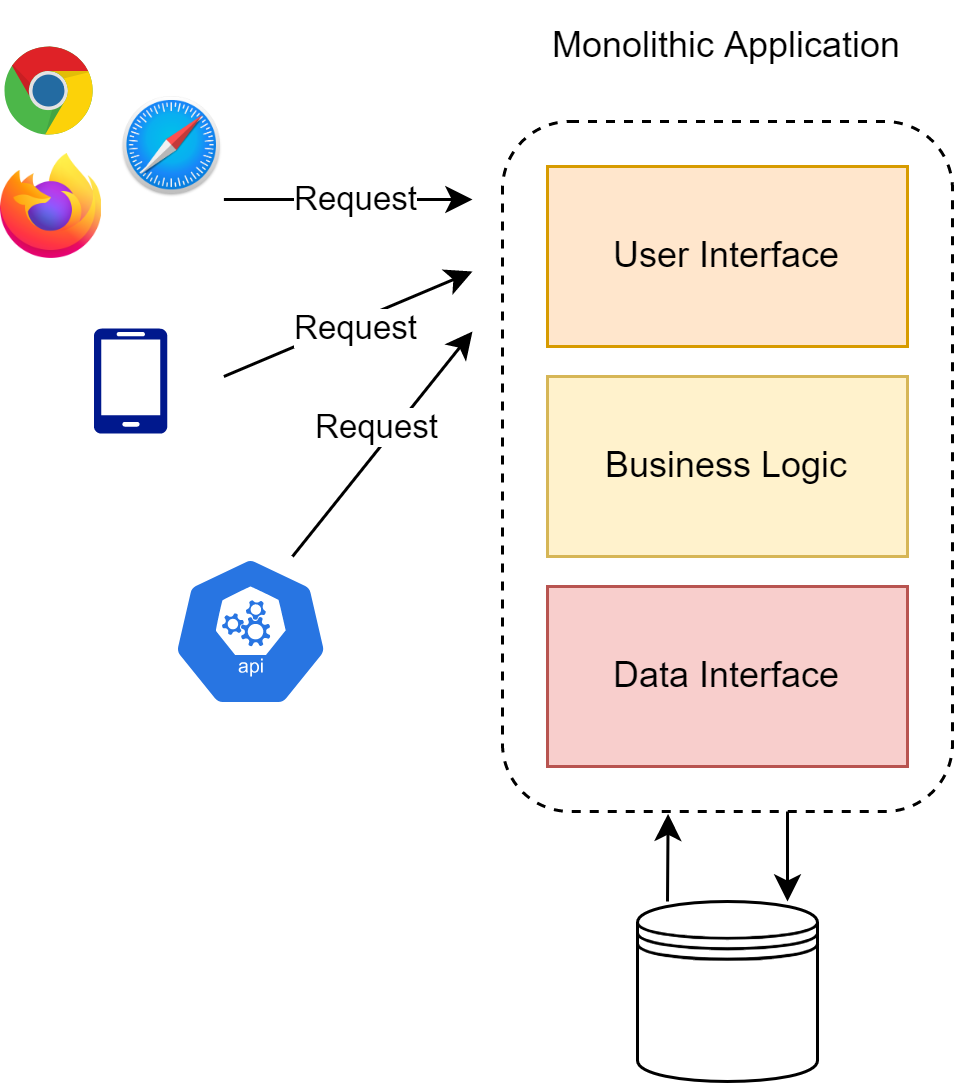
\includegraphics[width=0.7\linewidth]{img/Monolith.png}
 \end{center}
 \caption{Monolithic Architecture}
 \label{monolith}
\end{figure}

\noindent
A monolithic application has all services and business logic in one code base, which is being developed on. The development team need to ensure when modifying services that other parts of the application do not break. Monolithic architectures are common in many applications due to their simplicity and ability to meet system requirements quickly while limiting the number of dependencies that must be satisfied at deployment time. For example, e-commerce applications tend to use monolithic architectures because they are relatively simple and can be deployed quickly to achieve product/market fit. However, as the system scales, the system becomes increasingly complex to maintain and troubleshoot. Dependency management becomes increasingly difficult, and managing releases becomes challenging as changes have to be made across multiple layers in the system. A monolithic architecture also introduces a single point of failure that can adversely impact the entire system if it fails \cite{vil2015}.


\section{Microservice}
\begin{figure} [H]
 \begin{center}
    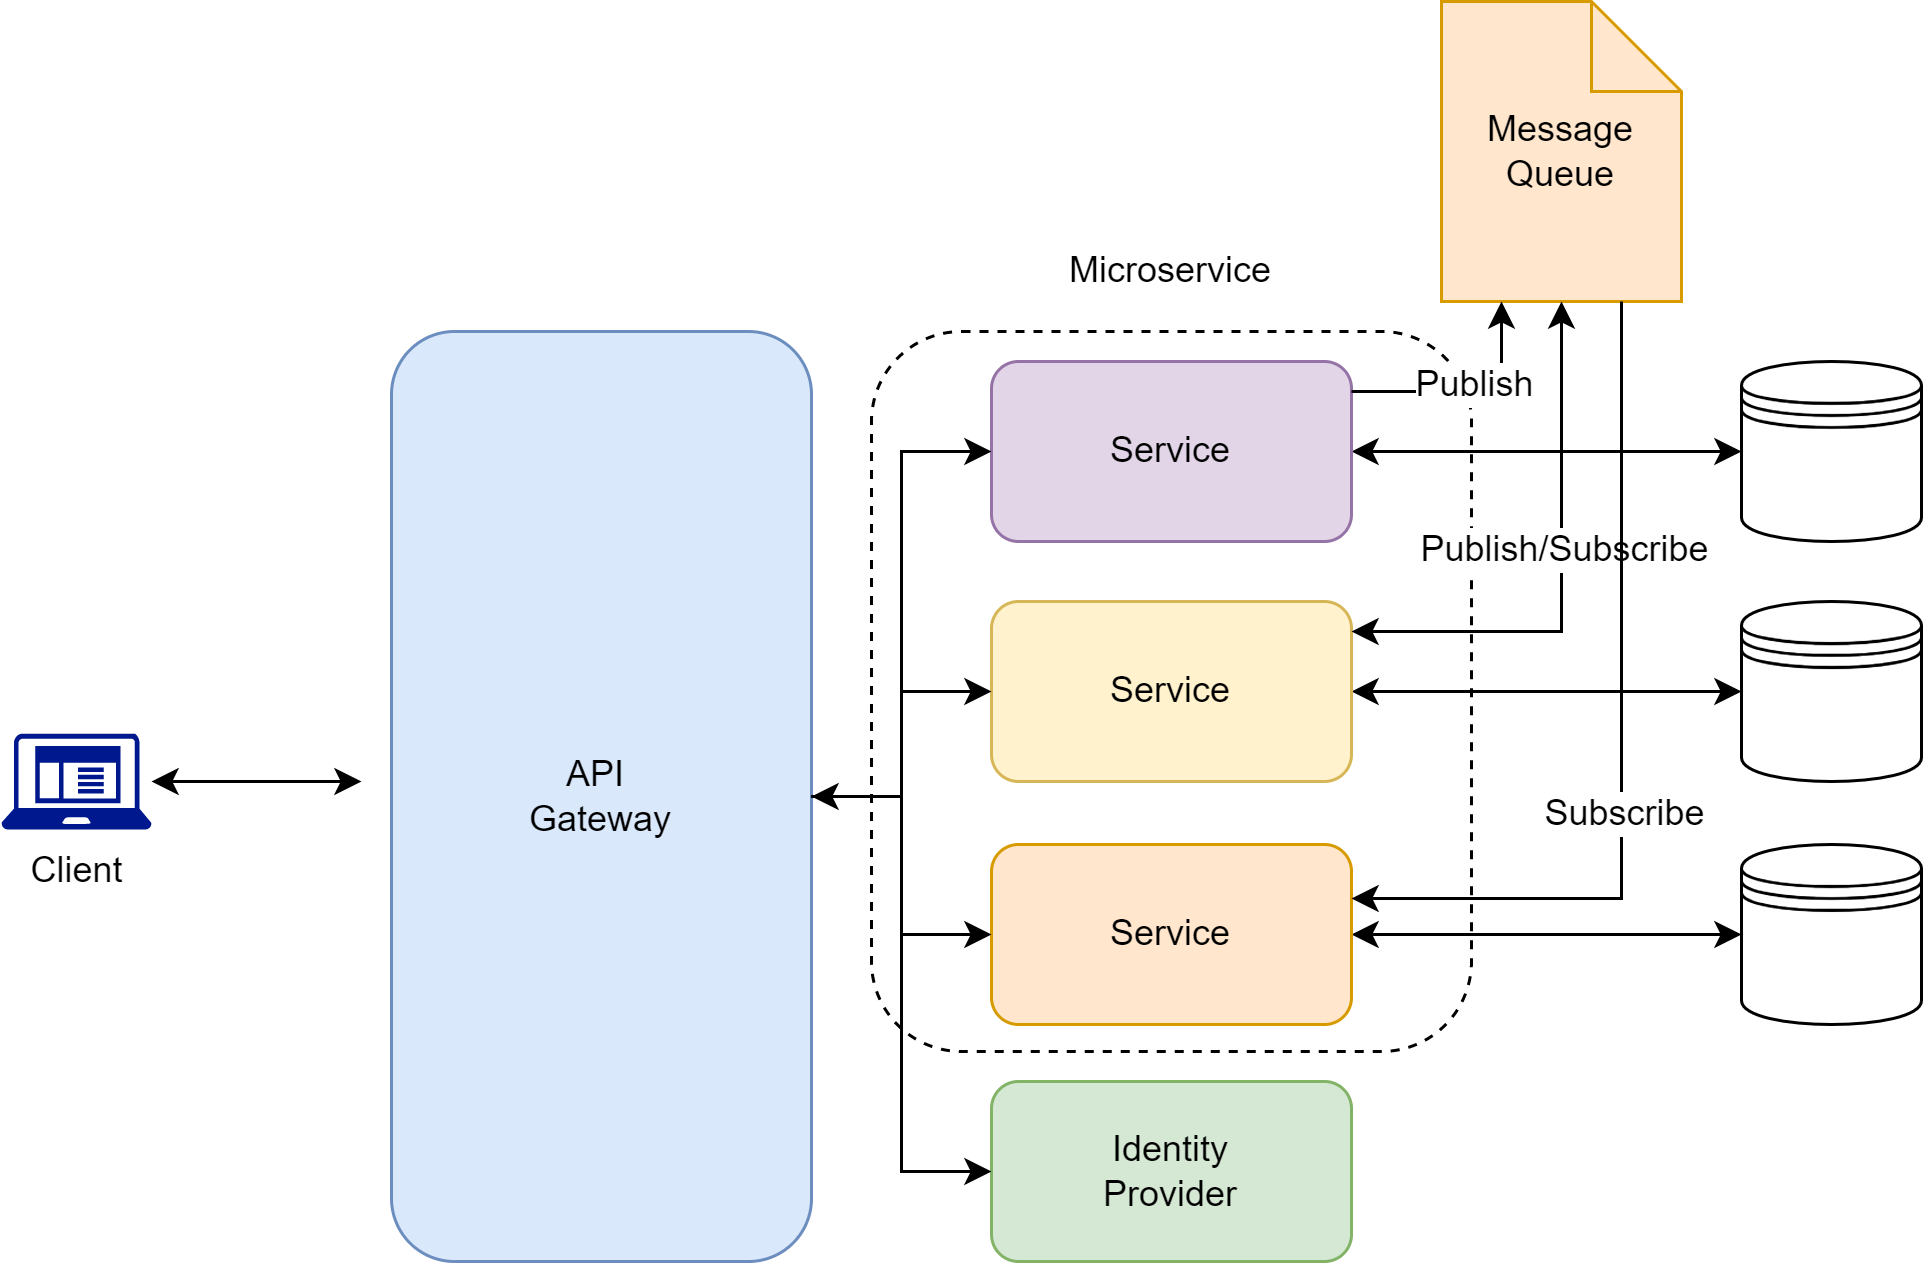
\includegraphics[width=1\linewidth]{img/Microservice.png}
 \end{center}
 \caption{Microservice Architecture}
 \label{microservice}
\end{figure}

\noindent
Microservices are separate, small, modular services that can be independently developed, updated, deployed and managed. Each service runs in its process and communicates over the network using a well-defined communication protocol \cite{fow2014}. These services are self-describing and can be discovered and used by other processes without human intervention. They are loosely coupled and can be easily scaled up and down based on the current business needs.
\\
\\
Microservices are a popular architectural style for building applications, where each service does one thing well. Each service typically only exposes a small set of its functionality via a RESTful API and communicates with other services using asynchronous messaging \cite{gooMes}. This style of architecture allows services to be scaled independently; if one service is overloaded, it can simply stop accepting new requests for some time without affecting the performance of other services.
\\
\\
Microservices are often built using API-first approaches, where the API is designed and developed first, followed by the other services that use it. This approach enables developers to prototype and tests the microservices in isolation before integrating them into the main application. This makes development and testing faster and more cost-effective. It also means that once a service is successfully deployed, it can be used in other contexts where it may be used to achieve additional benefits.
\\
\\
Microservices are a recent trend where each service can be developed independently and scaled independently, making it much faster to develop and deploy new versions or features with minimal downtime for the application users. On the other hand, a monolithic API approach is easier to maintain since it consists of a single process across the server instead of multiple processes that have to communicate over the network with each other \cite{pat2021}.
\\
\\
API management platforms[6] are tools which allow microservices to be managed easily. These tools allow the developer to work with different services and easily integrate them in the application by providing a uniform interface for the developers to communicate with each service. They provide tools for deploying and monitoring the services so they can easily be scaled up or down depending on the needs of the business.




\section{The Cloud}
By implementing DevOps practices in their organisations, companies can align IT operations with business goals and increase operational efficiency and agility. This is achieved by adopting new technologies like cloud computing, containerisation, microservices, and automation tools to speed up the development lifecycle and deliver high-quality products and services to customers faster. Companies can also reduce costs by optimising compute and storage consumption across different workloads and infrastructures \cite{qia2009}.

\subsection{Infrastracture as a Service (IaaS)}
Cloud providers such as AWS, Microsoft Azure, Google Cloud Platform, IBM Cloud, or Oracle Cloud provide cloud infrastructure-as-a-service (IaaS) that allows businesses to set up virtual machines on a shared infrastructure to manage their applications and workloads. IaaS is a cloud service that provides virtualised computing resources (e.g. CPU, memory, storage and networking resources) on demand to users over the Internet. It is managed by the service provider using a cloud computing stack that consists of the underlying hardware, virtualisation software and the cloud management platform \cite{buy2019} .
\\
\\
IaaS solutions enable companies to build and deploy their own custom IT systems on the cloud without having to purchase and maintain any hardware or software. It enables them to focus on building their applications and business processes without worrying about the technical details related to the IT infrastructure. IaaS also offers a lot of flexibility in terms of scaling up or down the resources required for their workloads as and when needed. It is still required to manage the OS and the package's whole deployment process.

\subsection{Platform as a Service (PaaS)}
Platform as a Service (PaaS) is a cloud computing service that provides a platform for developers to build and deploy their applications without worrying about the underlying infrastructure or hardware resources. 
\\
\\
The main benefits of using PaaS include the following: 

\begin{itemize}
\item Quick Setup and Deployment: With PaaS, developers no longer need to concern themselves with setting up and maintaining an IT infrastructure for running their applications, as all of this is done for them by the service provider. They can simply sign up for the service and start developing their application immediately and deploy it to the production environment by simply pushing a button without any further configuration or maintenance required. This can save a lot of time and effort on the developer's part so that they can focus on developing the application rather than troubleshooting technical issues \cite{law2008}.

\item Cost Effective: Eliminates the need to purchase and maintain expensive hardware and software resources for running applications and reduces the costs associated with managing such resources. Developers can use these services to develop their applications without investing in costly infrastructure components and equipment \cite{gai2014}.

\item High Availability: Helps cost-effectively achieve high availability by allowing users to scale their applications up or down depending on the requirements at any given time. With this service, they can easily scale down their applications when they are not required to increase efficiency and reduce costs. Similarly, they can scale up their applications when needed to provide additional capacity to handle increased workloads without incurring additional costs. In addition, the service provides them with various options to support different business requirements, such as the number of users, data storage requirements and bandwidth availability. This allows them to optimise the performance and functionality of their applications for different types of users. 

\item Scalability: Allows developers to easily scale their applications to accommodate growing workload requirements without making additional investments \cite{law2008}. They can do this by adding additional resources to their applications and scaling them up accordingly to meet the increasing demands. They can also easily scale their apps down when they are no longer required to reduce operational costs and minimise storage requirements.

\item Flexibility: Provides users with a high degree of flexibility in choosing their services and platform components to meet their specific needs. This gives them the ability to choose each component individually based on their specific requirements and only pay for the ones that they need. It also allows them to implement new features and functionality quickly and easily without requiring them to make any changes to the existing applications. 
\end{itemize}


\section{Docker}
Docker is an open-source platform for automating application containers on Linux based operating system. A Docker Container is lightweight, portable, and isolated application packaging. It allows developers to package an application and all its dependencies in a single file, known as a "container", that can run on any Linux server. Different containers can be combined into a single cluster, and each container runs as an independent process with its namespace. Docker containers are lightweight and can easily be moved between development and production environments. They can also easily be linked together to create powerful applications \cite{rad2017}.
\\
\\
The key benefits of using Docker Containers include the following: 

\begin{itemize}
\item Lightweight: Docker containers are generally smaller compared to a virtual machine. This means multiple applications can run on a single server without compromising performance.\cite{vmwcovsvm}

\item Portable: Docker containers are highly portable, which facilitates moving applications from development to production or even between different servers \cite{rad2017}. This is especially useful for DevOps teams as they can use the same containers in different environments, such as development and staging or production and testing.

\item Isolated: Each Docker container is completely isolated from other containers on the system, so there is less risk of a vulnerability affecting multiple containers simultaneously.\cite{com2016} This also helps to have multiple containers running different versions of runtimes or compilers, which would be much harder to maintain in a virtual machine.

\item Easy to Manage: Docker containers are designed to minimise management overhead so developers can focus on building great apps instead of managing infrastructure. This is achieved by giving the developer fine-grained control over container resources and providing simple tools for managing them. 

\item Secure and Reliable: Docker containers are more secure and reliable than traditional applications because they are self-contained and easy to manage. With Docker containers, a developer can use a different image for each environment and easily migrate their application between environments without running into any downtime or other issues. 

\item Efficient: Because Docker containers are easy to create and manage, they provide a cost-effective alternative to traditional applications that typically require complex and expensive infrastructure and management solutions. As a result, organisations can save a significant amount of time and money by moving to Docker containers for their development and deployment needs. 

\item High Performance: Containers provide a significant boost to the performance of any application by isolating it from the host machine. This means that each container can run independently of the others so that there are no resource constraints that can negatively affect its performance \cite{rad2017}.

\item Easily Scaled: Because containers run on the Linux kernel, they are easily scalable and highly customisable, which means that they can be configured to meet a wide range of performance and resource requirements \cite{rad2017}. In addition, they are compatible with most standard networking and storage technologies and can therefore be deployed in any environment. 
\end{itemize}

\noindent
Due to these advantages, Docker containers have become the de facto standard for deploying and running applications in the public cloud and have been widely adopted by both individual developers and large enterprises for all of their development and deployment needs.


\section{Kubernetes}
Kubernetes is open-source software for automating deployment, scaling and managing containerised applications. It provides a scalable way to run containerised applications on any public cloud or on-premise infrastructure. Kubernetes is workload agnostic, meaning that it can support multiple types of services without requiring the developers to re-architect the application for Kubernetes \cite{luk2018}.
\\
\\
Kubernetes features include resource provisioning, scalability, load balancing, service discovery, multi-cluster management, auto-scaling, etc. It also provides a REST API for managing resources and a web-based dashboard for end users to monitor the status of the cluster and the resources in it. These features enable Kubernetes to control and monitor many containers simultaneously in a dynamic environment. This enables it to be used as an Infrastructure as a Service (IaaS) platform for controlling and running applications in the cloud. It can also be used for development and testing environments as it can dynamically scale resources to meet user demand without deploying new servers each time additional resources are required \cite{kubernetes}.

\section{.NET}
//TODO überprüfen
\\
.NET Core is a free, open-source, and cross-platform framework for building modern applications. It was developed by Microsoft as a successor to the .NET Framework.
\\
\\
.NET Core is designed to be lightweight, modular, and efficient, making it suitable for building applications for a wide range of devices and workloads, including web applications, cloud services, and microservices. It can run on multiple operating systems, including Windows, Linux, and macOS.
\\
\\
.NET Core consists of a set of libraries and runtime components that provide the core functionality of the .NET Framework, such as support for data access, networking, and security. It also includes a cross-platform version of the Common Language Runtime (CLR), which is the runtime environment that executes .NET code.
\\
\\
.NET Core is built on top of the open-source .NET Foundation, which is a community-driven organization that oversees the development and evolution of the .NET ecosystem.

\section{API}
//TODO überprüfen
A Web API is a programming interface for building web applications. It is a collection of procedures, protocols, and tools for building software and applications.
\\
\\
A Web API allows for communication between different systems over HTTP, which is the standard protocol for exchanging data on the web. It enables a web application or service to expose its functionality to other systems over the web, using a set of predefined rules and standards.
\\
\\
Web APIs are often used to build web-based applications that need to interact with other systems or services. For example, a web-based email client might use a Web API to communicate with a mail server to send and receive email messages.
\\
\\
Web APIs are typically implemented using the HTTP protocol, which defines a set of methods (such as GET, POST, PUT, and DELETE) for interacting with resources on a server. A Web API can be consumed by a wide variety of clients, including web browsers, mobile devices, and desktop applications.
Quick intro:
https://dev.to/andreidascalu/soap-vs-rest-vs-grpc-vs-graphql-1ib6
Quick intro:
https://dev.to/andreidascalu/soap-vs-rest-vs-grpc-vs-graphql-1ib6
\subsection{Restful API}
\subsection{SOAP API}
\subsection{gRPC}
\subsection{graphQL}

\section{Swagger}


\clearpage
\chapter{Applied Methods}
The project created for this thesis called "Examich" is for students to create, manage and share practice exams. This service also offers the option to generate a PDF Version of the practice exams. Since this thesis focuses on the API the frontend for this project will be skipped.

\section{Monolith}

\subsection{Architecture \& Implementation}

\begin{figure} [H]
 \begin{center}
    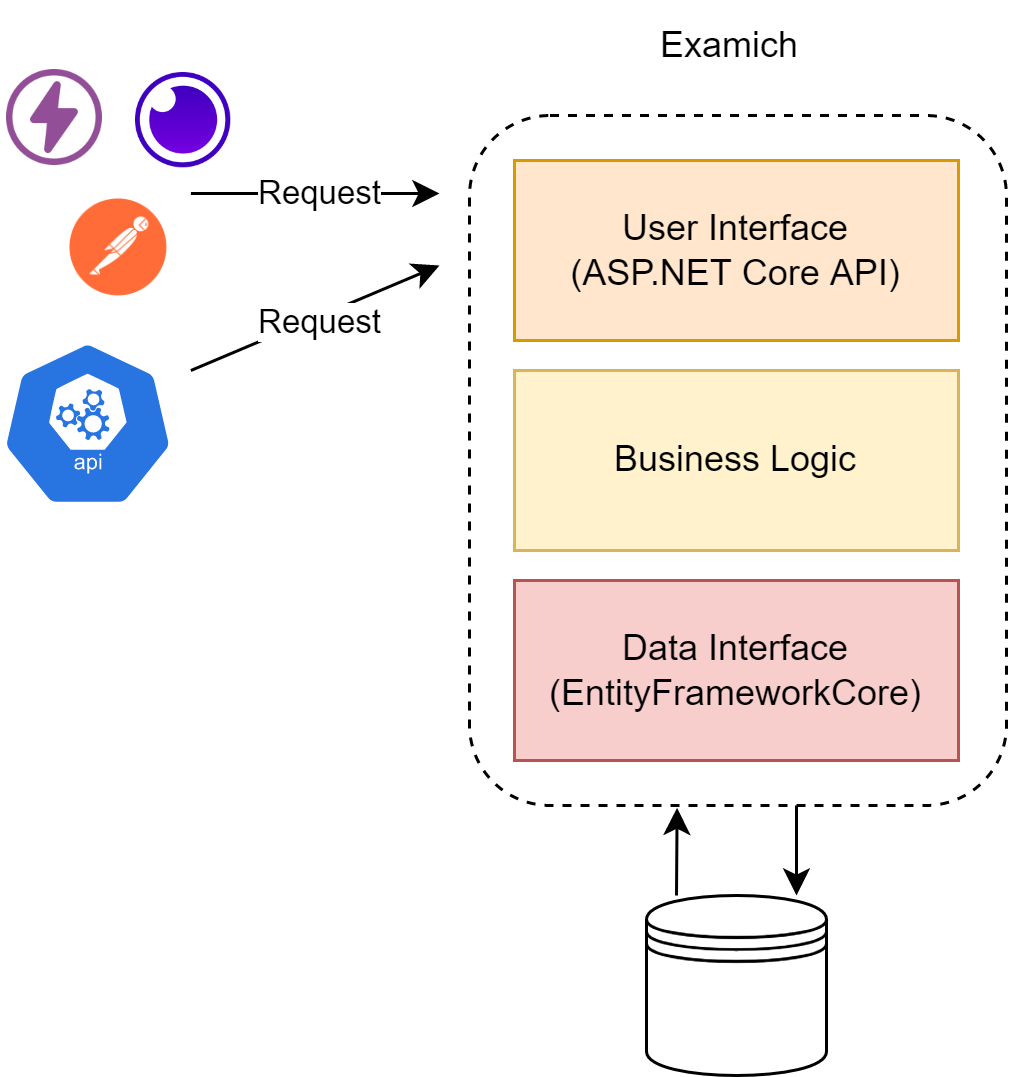
\includegraphics[width=0.6\linewidth]{img/ExamichMonolith.png}
 \end{center}
 \caption{Examich Monolith Architecture}
 \label{examichMonolith}
\end{figure}

The monolith consists of tree main parts. The API that exposes the functionality to its users. The business logic which does for now only handle the PDF Generation and the data layer which handles the communication with the data base.
\\
\noindent
The endpoints it exposes:

\begin{figure} [H]
 \begin{center}
    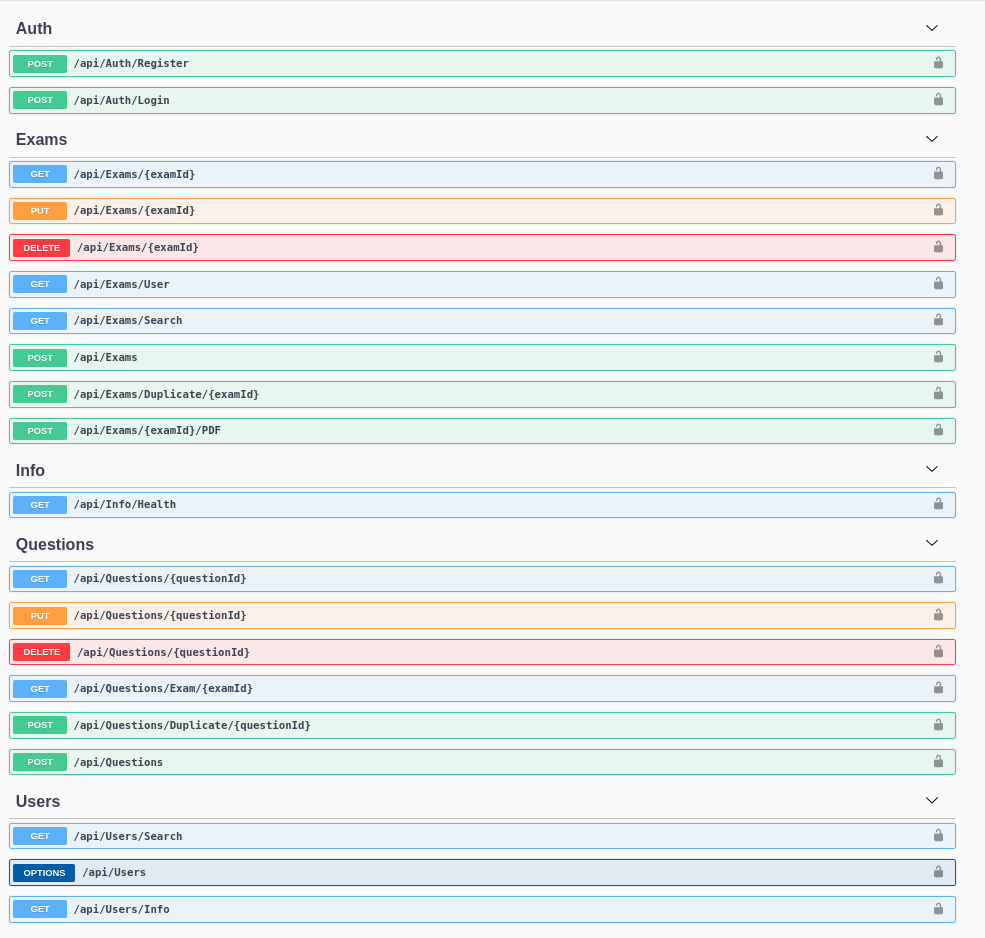
\includegraphics[width=0.8\linewidth]{img/Monolith_Swagger.png}
 \end{center}
 \caption{Examich Monolith Swagger}
 \label{examichMonolithSwagger}
\end{figure}
\noindent
The most resource intense endpoint would be "/api/Exams/{examId}/PDF", since with this the PDF generation is triggered. It will render the PDF and send it as response back to the user.


\subsection{Data Model}

\begin{figure} [H]
 \begin{center}
    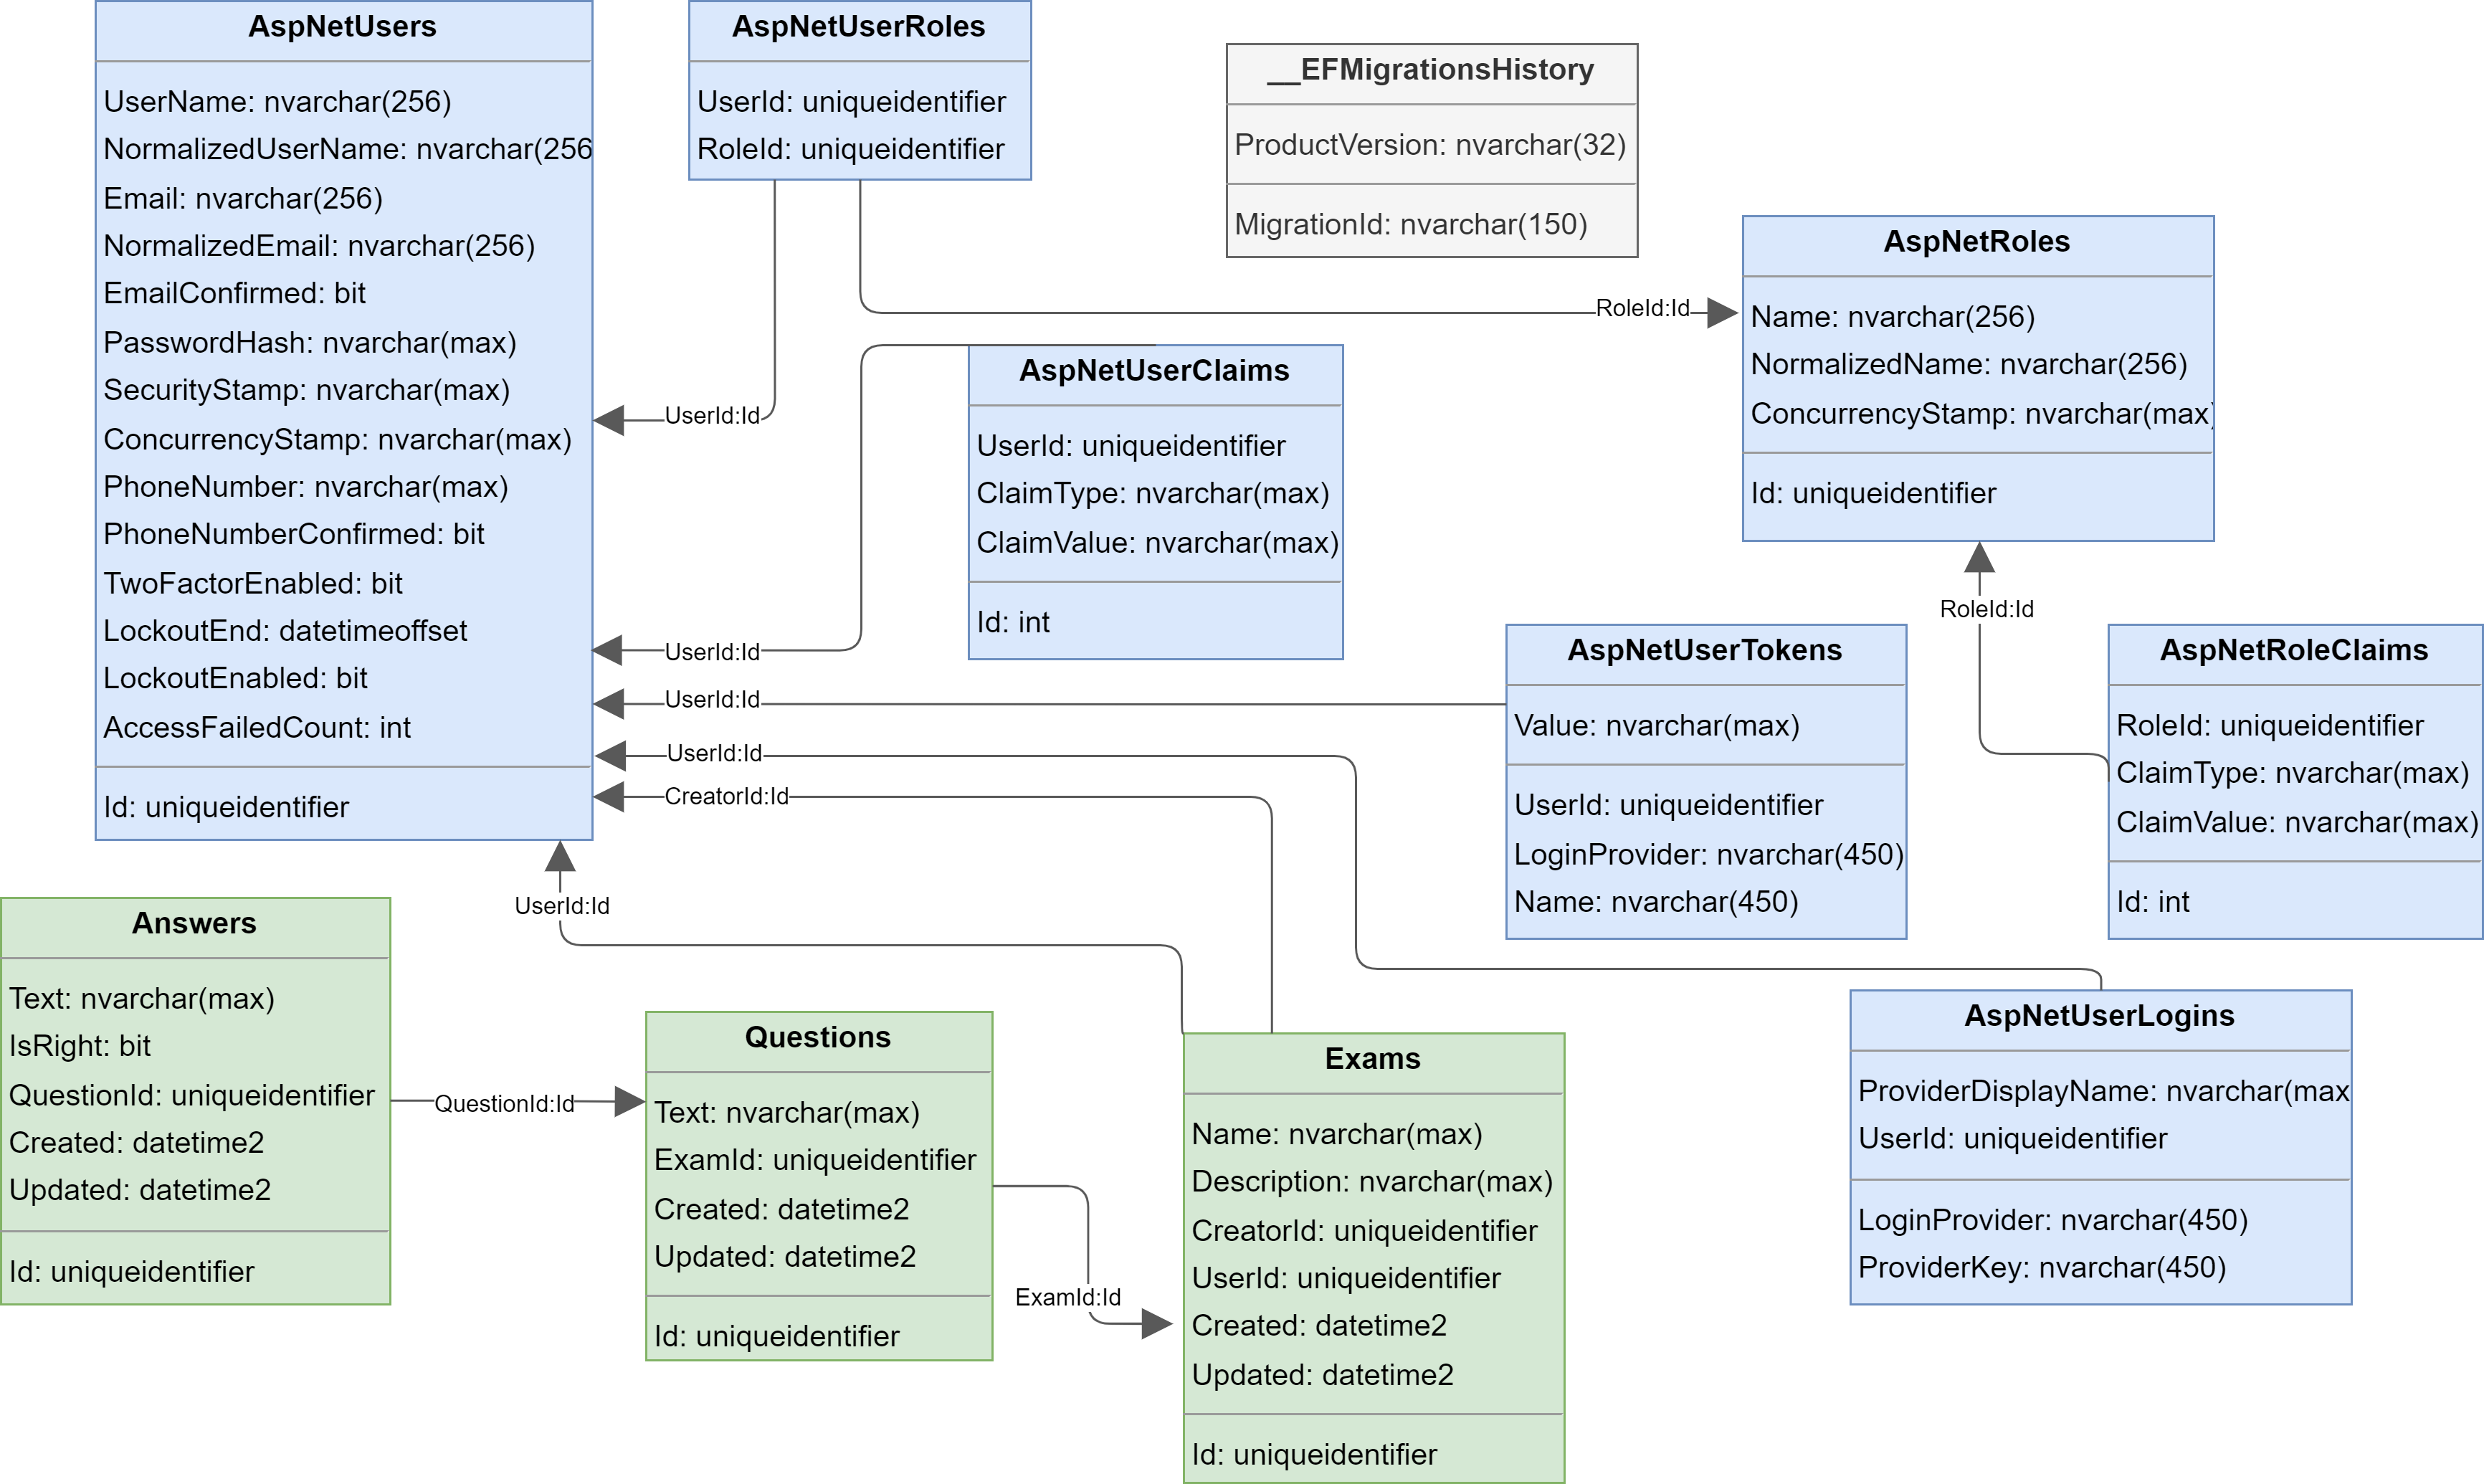
\includegraphics[width=1.1\linewidth]{img/ExamichDataModel.png}
 \end{center}
 \caption{Examich Monolith Data Model}
 \label{datamodel}
\end{figure}

This is the data model for the monolithic application. The blue tables are tables generated by the Microsoft.AspNetCore.Identity.EntityFrameworkCore.IdentityDbContext, the grey one is generated be EntitiyFrameworkCore to keep track of the migrations and the green ones were created for the project. The important tables are the green ones. Every User had zero or more Exams, every Exam had zero or more Questions and every Question had zero or more Answers. A pretty simple data structure.


\section{Microservice}

\subsection{Architecture \& Implementation}
\begin{figure} [H]
 \begin{center}
    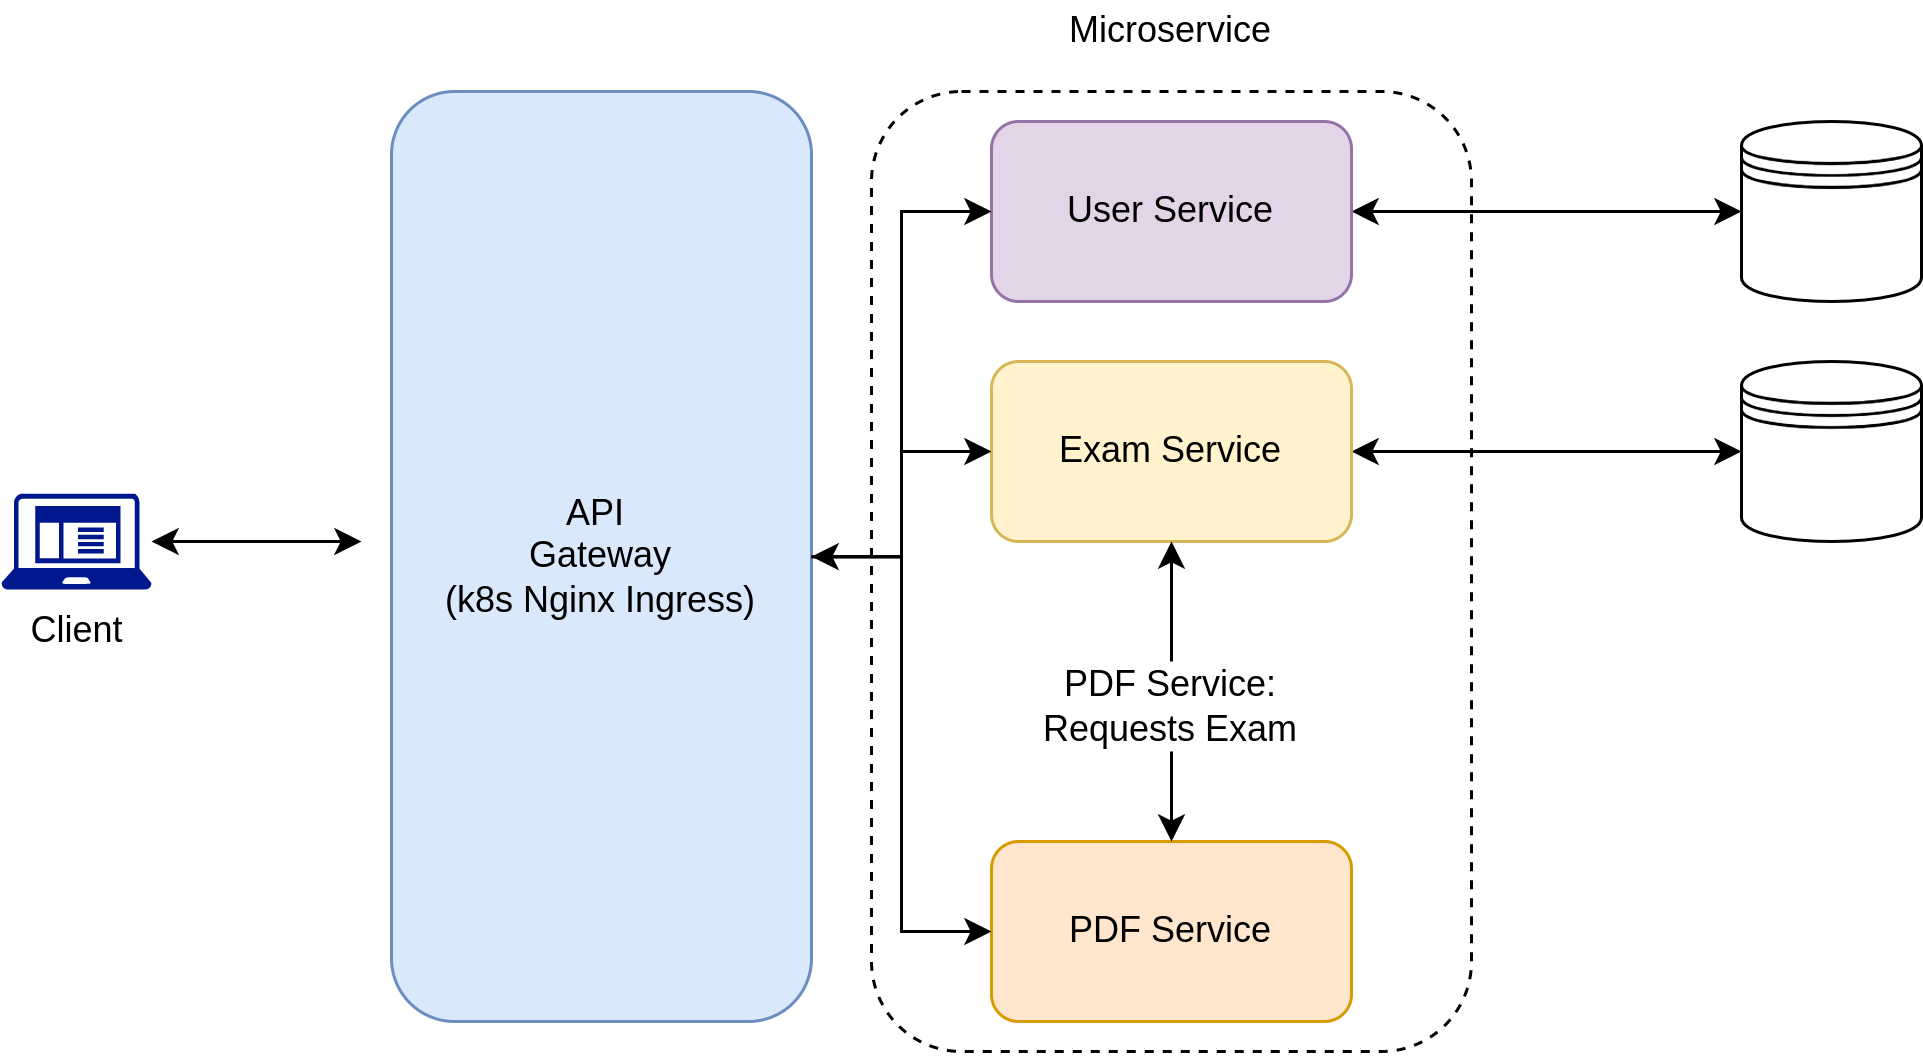
\includegraphics[width=1\linewidth]{img/ExamichMicroserviceArchitecture.png}
 \end{center}
 \caption{Examich Microservice Architecture}
 \label{examichMicroservice}
\end{figure}

\subsection{Data Model}

\begin{figure} [H]
 \begin{center}
    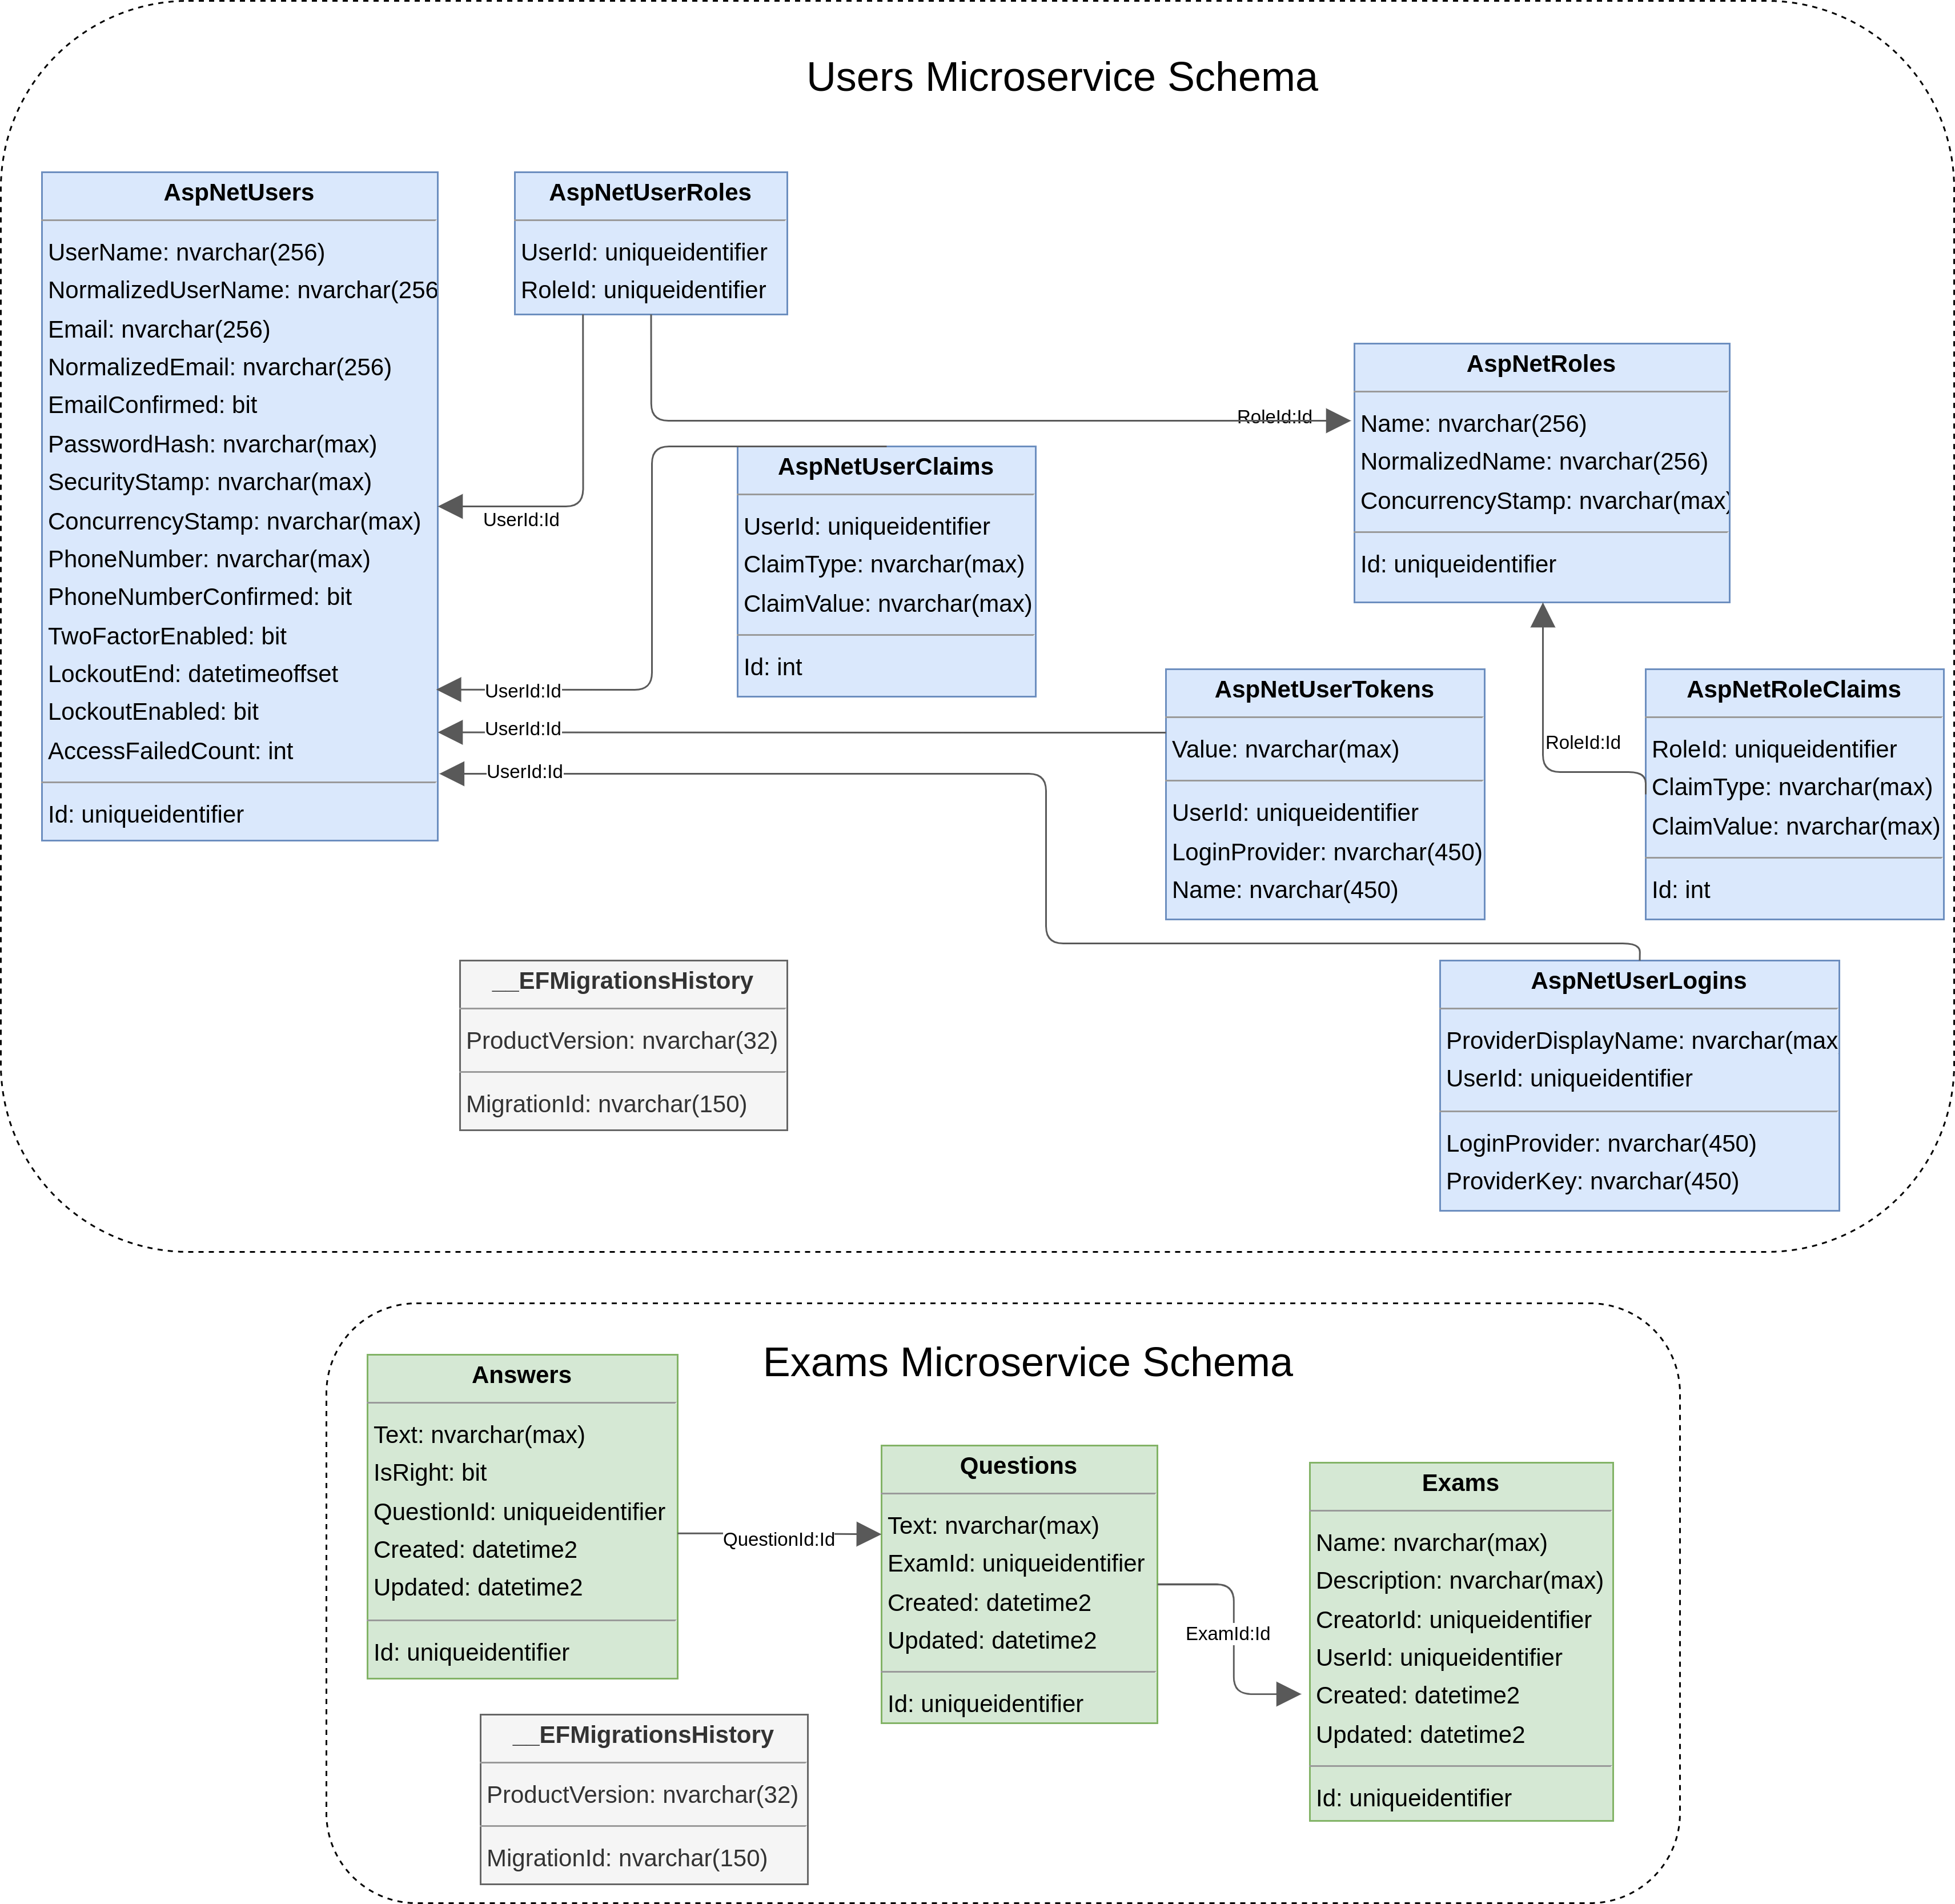
\includegraphics[width=1\linewidth]{img/ExamichMicroserviceDataModel.png}
 \end{center}
 \caption{Examich Microservice Data Model}
 \label{datamodelmicroservice}
\end{figure}




\section{Performance Benchmark}
This chapter will cover how the performance for the  monolith and microservice were tested.  

\subsection{k6 - Load Testing Tools}


\chapter{Results}

\section{Erste Überschrift Tiefe 2 (section)}

\subsection{Erste Überschrift Tiefe 3 (subsection)}

\subsubsection{Erste Überschrift Tiefe 4 (subsubsection)}


\chapter{Conclusion}

\section{Erste Überschrift Tiefe 2 (section)}

\subsection{Erste Überschrift Tiefe 3 (subsection)}

\subsubsection{Erste Überschrift Tiefe 4 (subsubsection)}


\subsubsection{Zweite Überschrift Tiefe 4 (subsubsection)}


\clearpage
\ifthenelse{\equal{\FHTWCitationType}{HARVARD}}{}{\bibliographystyle{gerabbrv}}
\bibliography{Literatur}
\clearpage

% Das Abbildungsverzeichnis
\listoffigures
\clearpage

\end{document}
